\documentclass[12pt,a4paper]{article}

\usepackage[utf8]{inputenc}
\usepackage[T1]{fontenc}
\usepackage[brazil]{babel}
\usepackage{geometry}
\usepackage{graphicx}
\usepackage{array}
\usepackage{booktabs}
\usepackage{longtable}
\usepackage{xcolor}
\usepackage{listings}
\usepackage{hyperref}
\usepackage{float}
\usepackage{setspace}
\usepackage{titlesec}

\geometry{left=3cm,right=2cm,top=3cm,bottom=2cm}
\onehalfspacing
\hypersetup{colorlinks=true,linkcolor=black,urlcolor=blue,citecolor=black}

\definecolor{codebg}{RGB}{245,247,250}
\definecolor{codeframe}{RGB}{210,220,230}
\definecolor{codeblue}{RGB}{20,65,110}

\lstdefinestyle{codigo}{
  backgroundcolor=\color{codebg},
  basicstyle=\ttfamily\footnotesize,
  breaklines=true,
  frame=single,
  rulecolor=\color{codeframe},
  keywordstyle=\color{codeblue}\bfseries,
  commentstyle=\color{gray},
  stringstyle=\color{purple},
  showstringspaces=false,
  tabsize=2
}
\lstset{style=codigo}

\titleformat{\section}{\normalfont\Large\bfseries}{\thesection}{1em}{}
\titleformat{\subsection}{\normalfont\large\bfseries}{\thesubsection}{1em}{}

\begin{document}

\begin{titlepage}
  \centering
  
\includegraphics[width=3.2cm]{figuras/logo-ueg.png}\par
  \vspace{1.2cm}
  {\large\bfseries UNIVERSIDADE ESTADUAL DE GOIÁS\par}
  \vspace{0.2cm}
  {\large Banco de Dados II\par}
  \vspace{2.2cm}
  {\Huge\bfseries Pokedex em Grafos com Docker\par}
  \vspace{0.5cm}
  {\Large Relatório Técnico Completo\par}
  \vspace{2.2cm}
  {\large\bfseries Integrantes\par}
  \vspace{0.4cm}
  {\large
  Kaique Vinícius Oliveira Alves\par
  Pedro Gabriel Mendes de Oliveira\par
  Gustavo Borges Sousa\par
  Peterson Silva Ribeiro\par
  Matheus Henrique do Couto\par
  }
  \vfill
  {\large 2026\par}
\end{titlepage}

\tableofcontents
\newpage

\section{Introdução}

Este relatório apresenta a aplicação \textit{Pokedex em Grafos}, desenvolvida com front-end em HTML, CSS e JavaScript, back-end em Node.js com Express e banco de dados Neo4j. O foco deste documento é explicar a parte de Docker do sistema: criação de imagem, execução de containers, uso de Docker Compose, configuração de rede personalizada, volumes persistentes e comandos básicos de validação.

O objetivo principal é demonstrar uma aplicação simples, empacotada em uma imagem Docker personalizada, executada em container e publicada em uma porta local. Também são demonstrados um container de banco de dados, comunicação entre aplicação e banco, persistência dos dados e evidências de execução por meio de comandos como \texttt{docker run}, \texttt{docker ps}, \texttt{docker images}, \texttt{docker stop} e \texttt{docker rm}.

\section{Fundamentação Teórica}

Docker é uma plataforma de containerização que permite empacotar uma aplicação e suas dependências em unidades chamadas containers. Um container executa a aplicação em um ambiente isolado, o que facilita a reprodução do sistema em diferentes computadores.

Uma imagem Docker funciona como um modelo usado para criar containers. Essa imagem é construída a partir de um arquivo chamado \texttt{Dockerfile}, no qual são descritos a imagem base, as dependências, os arquivos copiados e o comando de inicialização da aplicação.

Docker Compose é uma ferramenta que permite declarar múltiplos serviços em um único arquivo \texttt{docker-compose.yml}. No projeto, o Compose automatiza a execução da aplicação e do banco Neo4j, além de configurar portas, variáveis de ambiente, rede e volumes.

Redes Docker permitem que containers se comuniquem entre si pelo nome do serviço. Volumes Docker permitem persistir dados mesmo que o container seja reiniciado ou recriado, o que é essencial para o container do banco Neo4j.

\section{Descrição da Aplicação}

A aplicação é uma Pokedex em Grafos. Ela permite consultar Pokémon, visualizar relações de tipo, evolução, fraquezas e habilidades, além de usar uma área do treinador para login, favoritos e equipes.

O front-end foi construído com HTML, CSS e JavaScript puro. Em produção, ele é compilado e copiado para dentro da imagem da aplicação. O back-end é uma API em Node.js com Express, responsável por receber requisições HTTP, validar dados, autenticar usuários e acessar o banco Neo4j.

O Neo4j foi escolhido porque o domínio da Pokedex possui muitos relacionamentos. Pokémon se relacionam com tipos, fraquezas, habilidades, evoluções, usuários e equipes. Essa estrutura combina com o modelo de nós e relacionamentos de um banco de grafos.

\section{Explicação do Dockerfile}

O Dockerfile do projeto utiliza duas etapas. A primeira etapa compila o front-end com Vite. A segunda etapa instala o back-end em modo produção, copia o back-end e inclui o build final do front-end.

\begin{lstlisting}[language=Dockerfile]
FROM node:20-alpine AS frontend-build
WORKDIR /app/frontend
COPY frontend/package*.json ./
RUN npm ci
COPY frontend/ ./
RUN npm run build

FROM node:20-alpine AS app
WORKDIR /app
ENV NODE_ENV=production
COPY backend/package*.json ./backend/
RUN cd backend && npm ci --omit=dev
COPY backend ./backend
COPY --from=frontend-build /app/frontend/dist ./frontend/dist
WORKDIR /app/backend
EXPOSE 3000
CMD ["npm", "start"]
\end{lstlisting}

A instrução \texttt{FROM node:20-alpine AS frontend-build} inicia a etapa de build do front-end. A imagem \texttt{node:20-alpine} é uma versão leve do Node.js. Em seguida, o comando \texttt{WORKDIR} define a pasta de trabalho, os arquivos de dependências são copiados e \texttt{npm ci} instala as dependências de forma reproduzível.

Após copiar o código do front-end, o comando \texttt{npm run build} gera a pasta final de produção. Na segunda etapa, o Dockerfile cria a imagem final da aplicação. O back-end é instalado com \texttt{npm ci --omit=dev}, evitando dependências de desenvolvimento. A linha \texttt{COPY --from=frontend-build} copia o front-end já compilado para dentro da imagem final.

Por fim, \texttt{EXPOSE 3000} documenta a porta utilizada pela aplicação, e \texttt{CMD ["npm", "start"]} define o comando executado quando o container inicia.

\section{Explicação do Docker Compose}

O arquivo \texttt{docker-compose.yml} define os serviços necessários para executar o sistema completo.

\begin{lstlisting}
services:
  neo4j:
    image: neo4j:5-community
    container_name: pokedex-neo4j
    environment:
      NEO4J_AUTH: neo4j/pokedex123
    ports:
      - "7474:7474"
      - "7687:7687"
    volumes:
      - neo4j_data:/data
      - neo4j_logs:/logs
    networks:
      - pokedex_net

  app:
    build: .
    container_name: pokedex-app
    depends_on:
      - neo4j
    restart: on-failure
    environment:
      PORT: 3000
      NEO4J_URI: bolt://neo4j:7687
      NEO4J_USER: neo4j
      NEO4J_PASSWORD: pokedex123
      JWT_SECRET: pokedex_backend_dev_secret_2026
    ports:
      - "3000:3000"
    networks:
      - pokedex_net
\end{lstlisting}

O serviço \texttt{neo4j} utiliza a imagem oficial \texttt{neo4j:5-community}. Ele publica a porta 7474 para acesso ao Neo4j Browser e a porta 7687 para comunicação via protocolo Bolt. Também possui volumes para dados e logs.

O serviço \texttt{app} é construído a partir do Dockerfile do projeto. Ele depende do Neo4j, publica a porta 3000 e recebe variáveis de ambiente para configurar a API. A URI \texttt{bolt://neo4j:7687} usa o nome do serviço \texttt{neo4j}, pois os containers se comunicam dentro da rede Docker personalizada.

\section{Redes e Volumes Utilizados}

O projeto utiliza uma rede personalizada chamada \texttt{pokedex\_net}. Essa rede permite que o container da aplicação encontre o container do Neo4j pelo nome do serviço. Assim, dentro do container \texttt{pokedex-app}, o banco é acessado como \texttt{neo4j}, e não como \texttt{localhost}.

Os volumes utilizados são \texttt{neo4j\_data} e \texttt{neo4j\_logs}. O volume \texttt{neo4j\_data} armazena os dados do banco. O volume \texttt{neo4j\_logs} armazena logs do Neo4j. A persistência em volume é importante porque containers podem ser removidos e recriados, mas os dados devem continuar disponíveis.

\begin{lstlisting}
volumes:
  neo4j_data:
  neo4j_logs:

networks:
  pokedex_net:
    driver: bridge
\end{lstlisting}

\section{Comandos Utilizados}

Para subir todo o ambiente, foi utilizado:

\begin{lstlisting}
docker compose up --build
\end{lstlisting}

Para listar os containers em execução:

\begin{lstlisting}
docker ps
\end{lstlisting}

Para listar imagens:

\begin{lstlisting}
docker images
\end{lstlisting}

Para testar a execução básica do Docker:

\begin{lstlisting}
docker run --rm hello-world
\end{lstlisting}

Para testar parada e remoção de container sem derrubar a aplicação principal:

\begin{lstlisting}
docker run --name teste-stop-rm -d node:20-alpine tail -f /dev/null
docker ps --filter name=teste-stop-rm
docker stop teste-stop-rm
docker rm teste-stop-rm
\end{lstlisting}

Para conferir rede e volumes:

\begin{lstlisting}
docker network ls --filter name=pokedex
docker volume ls --filter name=pokedex
\end{lstlisting}

\section{Demonstração da Aplicação}

Após subir o ambiente, a aplicação fica disponível em:

\begin{lstlisting}
http://localhost:3000/app
\end{lstlisting}

O Neo4j Browser fica disponível em:

\begin{lstlisting}
http://localhost:7474
\end{lstlisting}

No Neo4j Browser, é possível executar a consulta abaixo para visualizar os nós e relacionamentos:

\begin{lstlisting}
MATCH (n)-[r]->(m) RETURN n, r, m LIMIT 50;
\end{lstlisting}

\section{Evidências de Execução}

\begin{figure}[H]
\centering
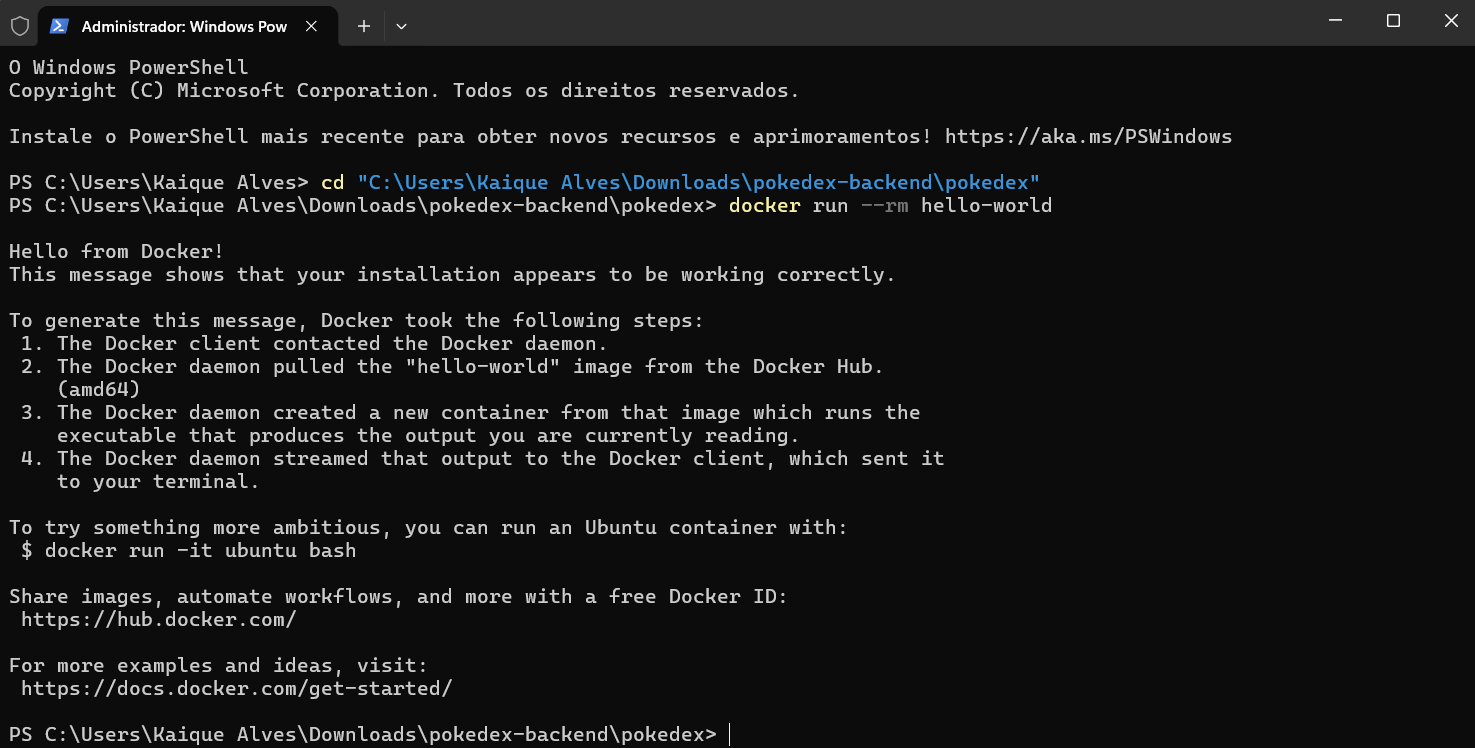
\includegraphics[width=\textwidth]{figuras/docker-hello-world.png}
\caption{Execução do comando \texttt{docker run --rm hello-world}.}
\end{figure}

\begin{figure}[H]
\centering
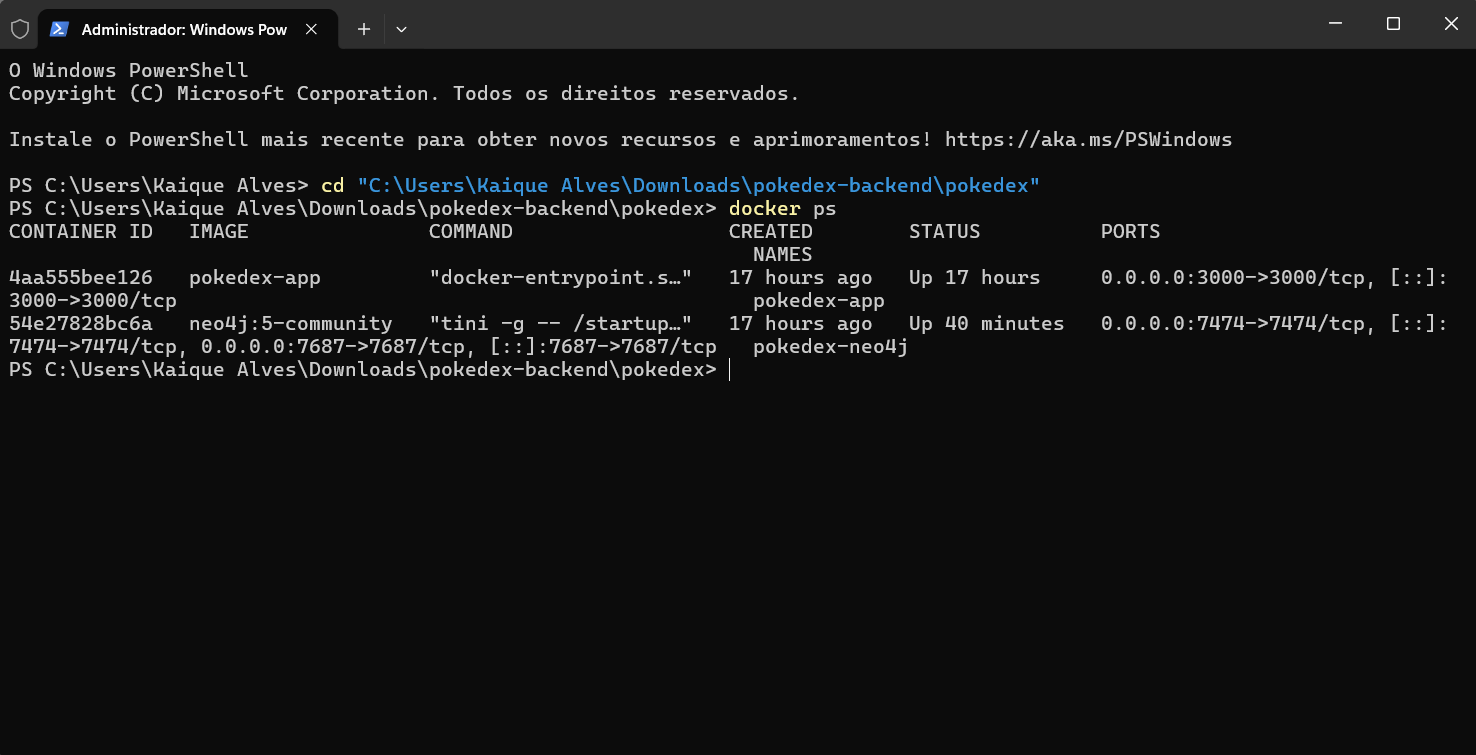
\includegraphics[width=\textwidth]{figuras/docker-ps.png}
\caption{Containers \texttt{pokedex-app} e \texttt{pokedex-neo4j} em execução.}
\end{figure}

\begin{figure}[H]
\centering
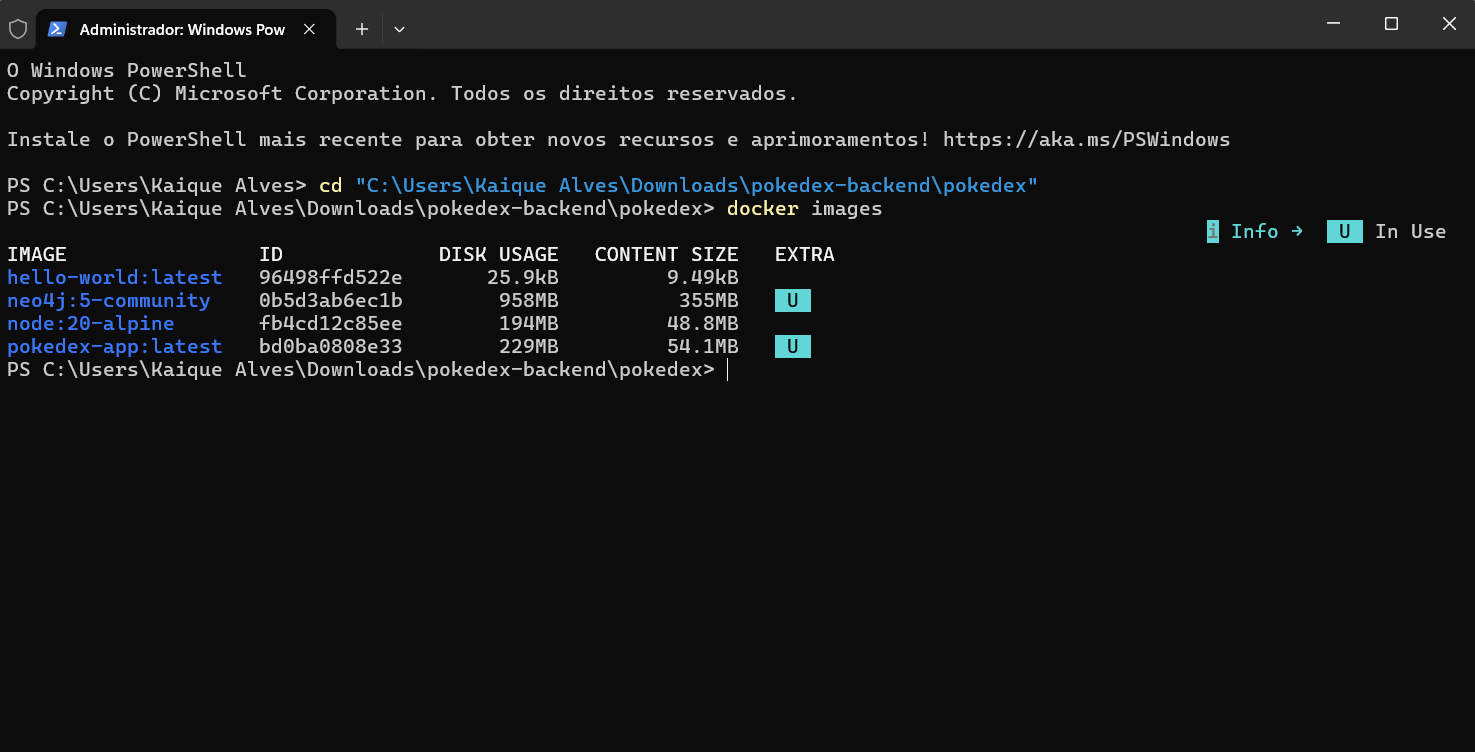
\includegraphics[width=\textwidth]{figuras/docker-images.png}
\caption{Imagens Docker disponíveis, incluindo \texttt{pokedex-app}.}
\end{figure}

\begin{figure}[H]
\centering
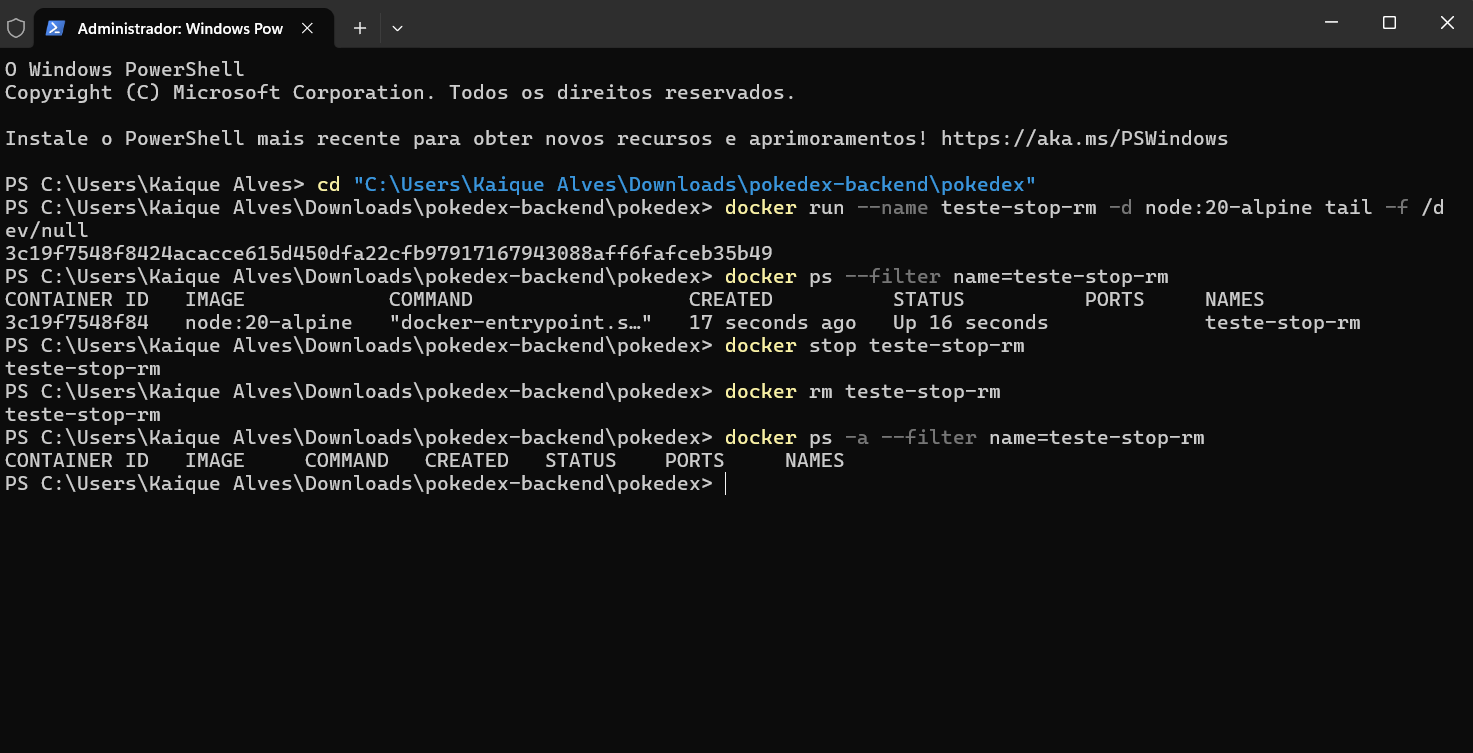
\includegraphics[width=\textwidth]{figuras/docker-run-stop-rm.png}
\caption{Teste com \texttt{docker run}, \texttt{docker stop} e \texttt{docker rm}.}
\end{figure}

\begin{figure}[H]
\centering
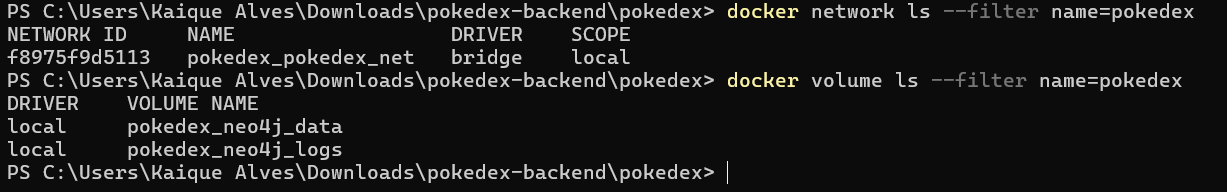
\includegraphics[width=\textwidth]{figuras/docker-network-volume.png}
\caption{Rede personalizada e volumes persistentes do projeto.}
\end{figure}

\begin{figure}[H]
\centering
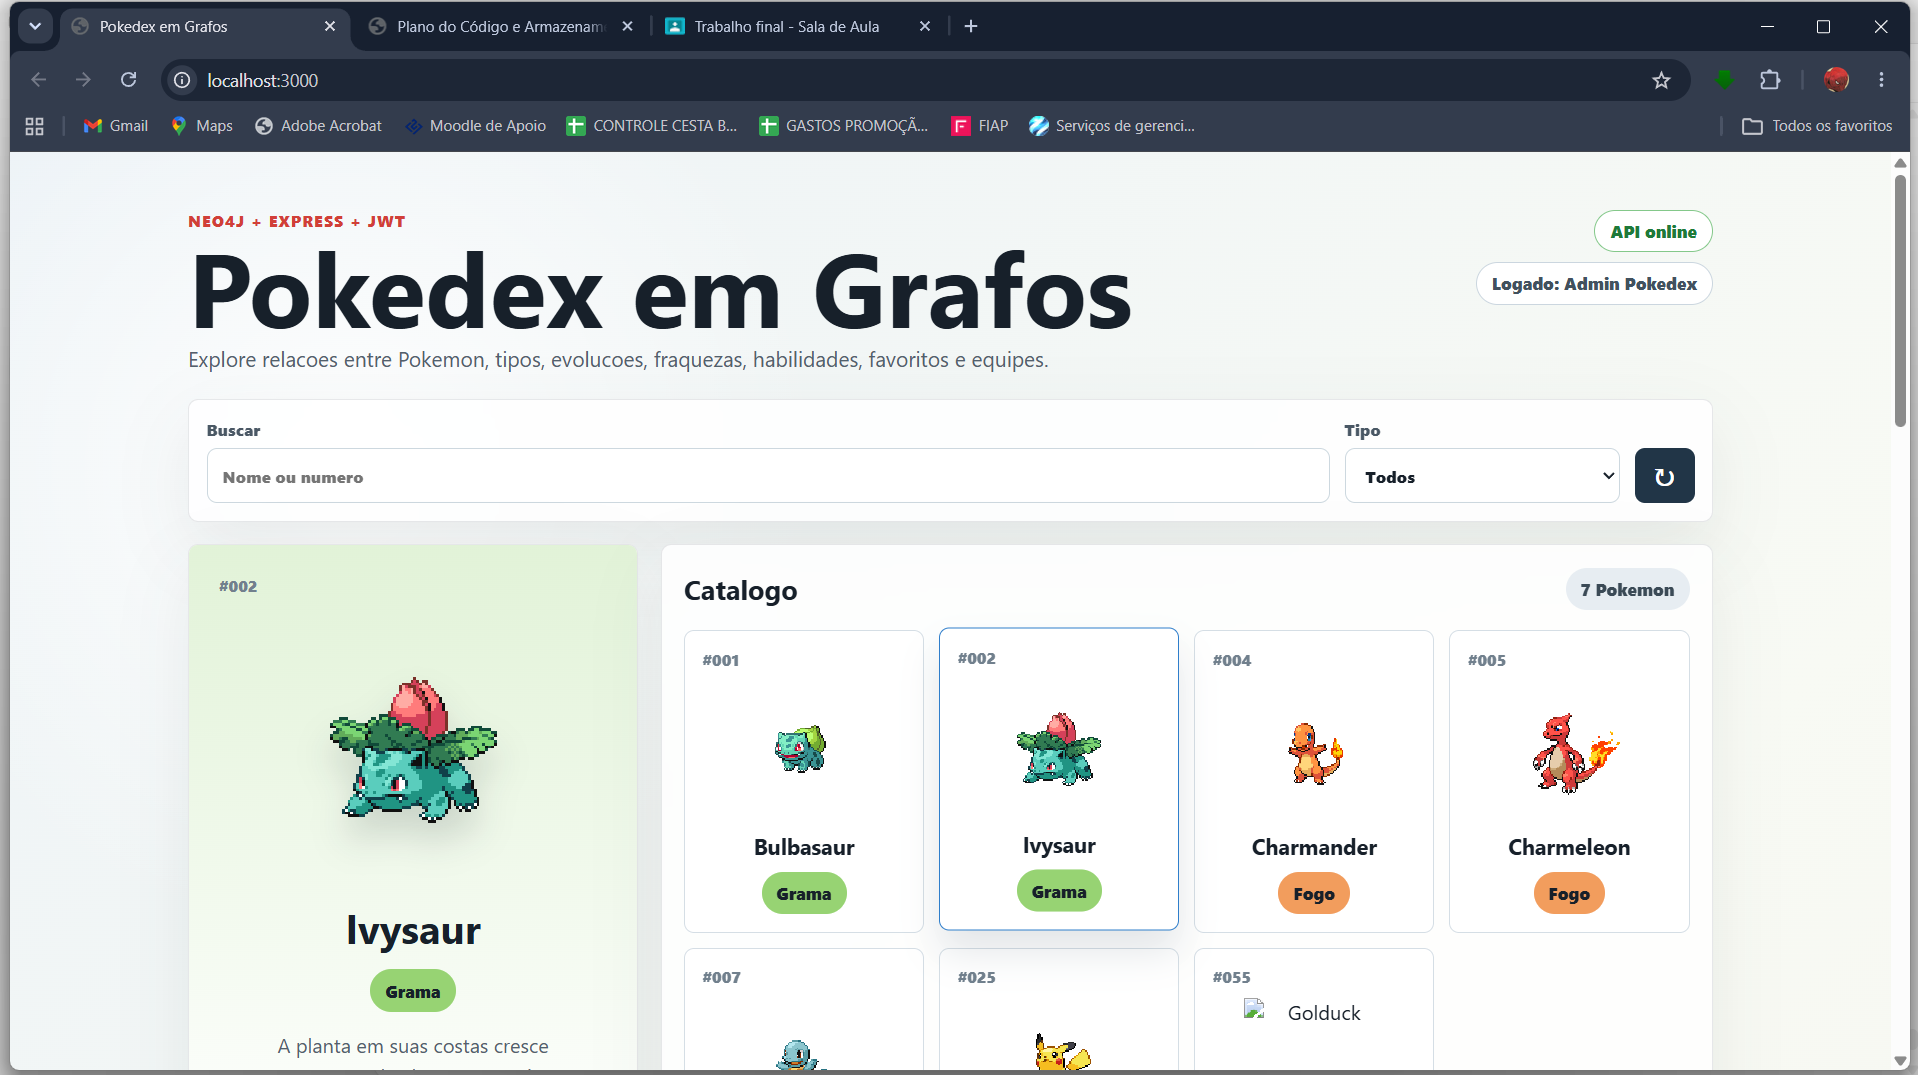
\includegraphics[width=\textwidth]{figuras/app-interface.png}
\caption{Interface da Pokedex em Grafos funcionando no navegador.}
\end{figure}

\begin{figure}[H]
\centering
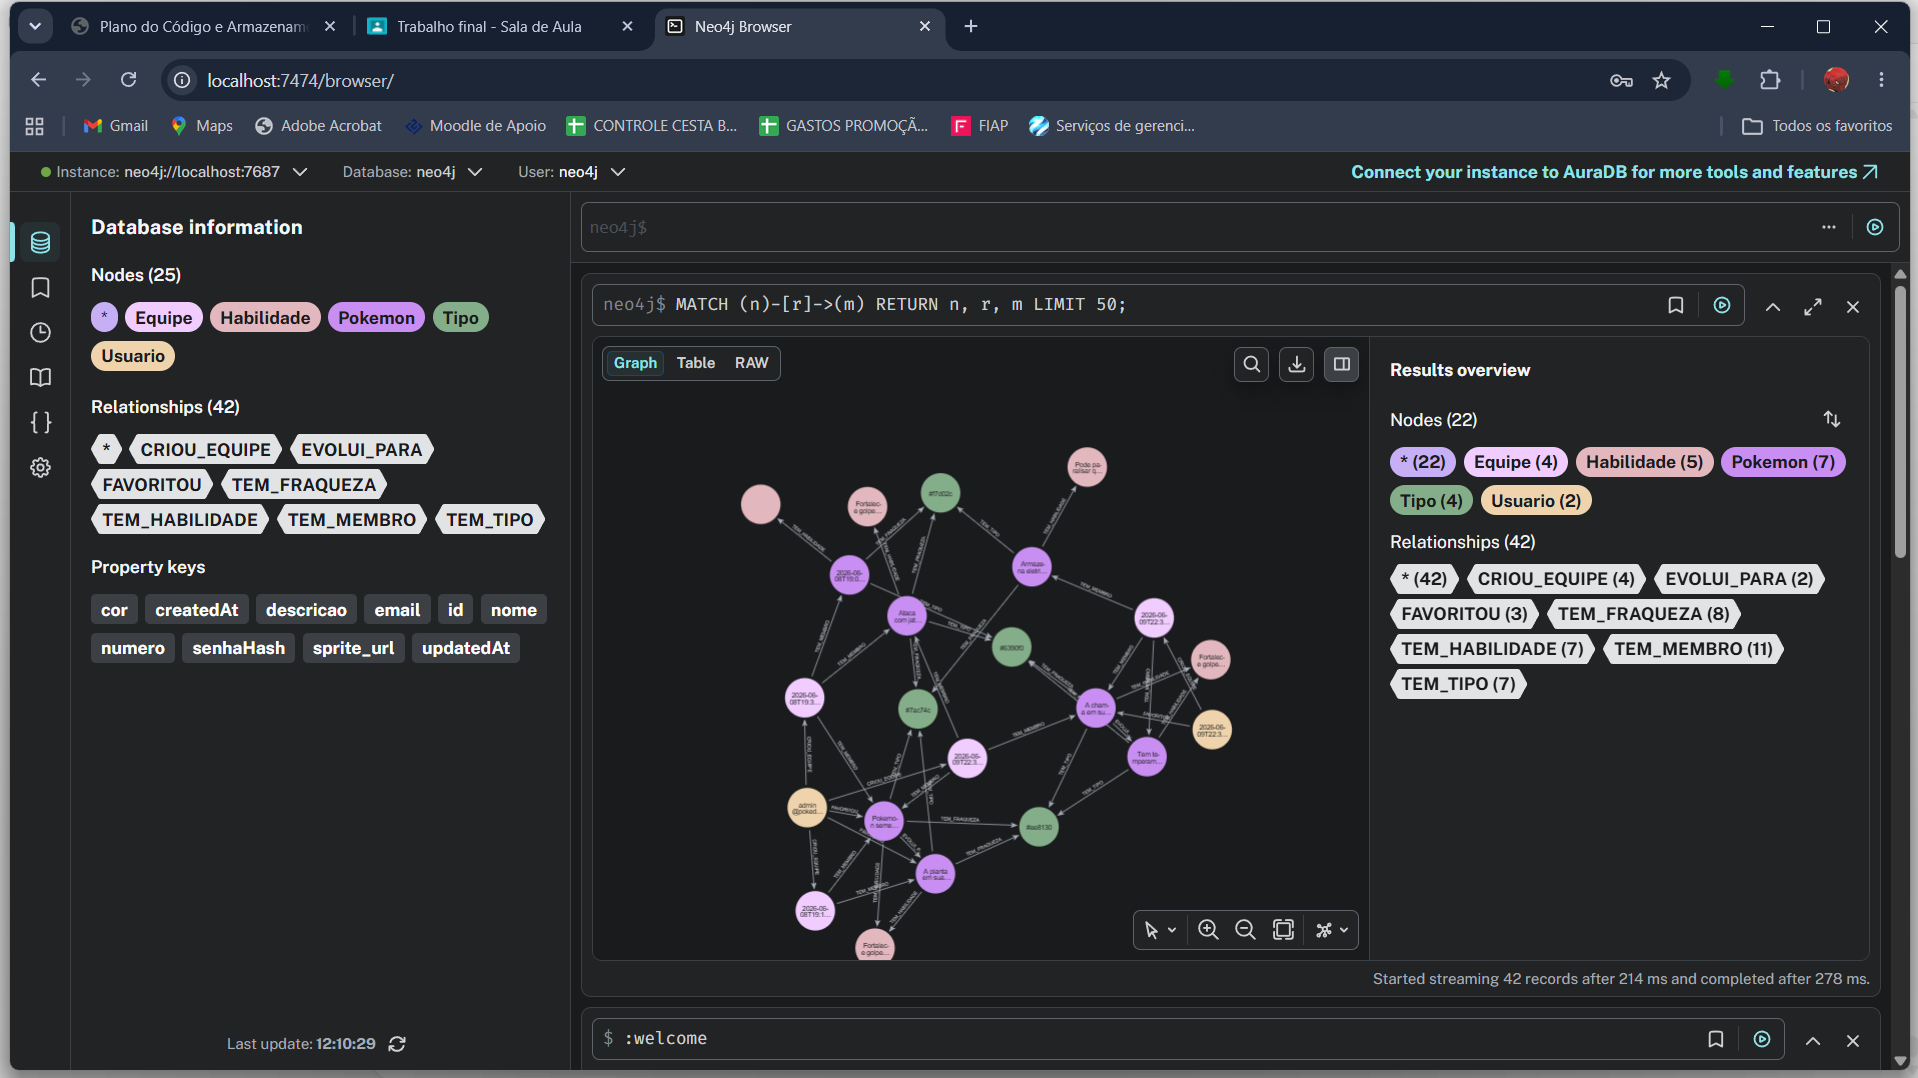
\includegraphics[width=\textwidth]{figuras/neo4j-browser.png}
\caption{Neo4j Browser exibindo nós e relacionamentos do grafo.}
\end{figure}

\section{Dificuldades Encontradas}

Durante o desenvolvimento e execução do ambiente, ocorreram dificuldades relacionadas à configuração do Docker Desktop. Em um primeiro momento, o comando \texttt{docker} não era reconhecido no terminal. Depois, houve erro de conexão com o Docker Engine, indicando que o serviço do Docker não estava em execução.

Também ocorreu erro de tempo de conexão ao tentar baixar a imagem \texttt{node:20-alpine} do Docker Hub. Esse erro foi relacionado à conexão de rede e foi resolvido ao tentar novamente após o Docker estar corretamente iniciado.

Outro ponto observado foi que o container da aplicação poderia tentar conectar ao Neo4j antes de o banco estar completamente pronto. Para reduzir esse problema, o back-end foi preparado para aguardar a conexão com o banco e o serviço \texttt{app} recebeu \texttt{restart: on-failure}.

\section{Conclusão}

O sistema Pokedex em Grafos atende aos requisitos relacionados à criação de uma aplicação simples, Dockerfile funcional, imagem personalizada, execução em container e publicação em porta local. Além disso, o ambiente possui dois serviços principais, aplicação e banco Neo4j, configurados por Docker Compose.

O projeto também utiliza rede personalizada, volumes persistentes e variáveis de ambiente. A aplicação é acessada pela porta 3000, enquanto o Neo4j é acessado pelas portas 7474 e 7687. As evidências apresentadas demonstram a execução dos principais comandos Docker e o funcionamento do sistema no navegador e no Neo4j Browser.

\section{Referências}

DOCKER. \textit{Docker Documentation}. Disponível em: \url{https://docs.docker.com/}. Acesso em: 10 jun. 2026.

NEO4J. \textit{Neo4j Documentation}. Disponível em: \url{https://neo4j.com/docs/}. Acesso em: 10 jun. 2026.

NODE.JS. \textit{Node.js Documentation}. Disponível em: \url{https://nodejs.org/docs/latest/api/}. Acesso em: 10 jun. 2026.

EXPRESS. \textit{Express - Node.js web application framework}. Disponível em: \url{https://expressjs.com/}. Acesso em: 10 jun. 2026.

\end{document}
